
\documentclass[cn,normal,black,11pt]{elegantnote}
\usepackage{wasysym}
\usepackage{multirow}
\usepackage{listings}

\begin{document}
\newcommand{\stuname}{陈鹏宇}
\newcommand{\stuclass}{2020级计算机科学与技术01班}
\newcommand{\name}{徐小龙}
\newcommand{\class}{2020级计算机科学与技术02班}
\newcommand{\expname}{实验一 简单流水线与运算器实验}
\newcommand{\expdate}{2022 年 04 月 16 日}
\newcommand{\reportdate}{\number\year 年 \number\month 月 \number\day 日}
\newcommand{\exproom}{Ds1410}
\newcommand{\stugrade}{优秀/良好/中等}
\newcommand{\teacher}{钟将}

\setlist[itemize]{label=$\circ$}

\centerline{\textbf{\huge{《计算机组成原理》实验报告}}}


\begin{table}[htbp]
    \centering
    \begin{tabular}{|c|c|c|c|}
        \hline
         \textbf{年级、专业、班级} & \stuclass & \textbf{姓名} & \stuname  \\
         \textbf{} & \class & \textbf{} & \name  \\ \hline
         \textbf{实验题目} & \multicolumn{3}{c|}{\expname} \\ 
         \hline
         \textbf{实验时间} & \expdate & \textbf{实验地点} & \exproom \\ \hline
\multirow{3}{*}{\textbf{实验成绩}} & \multirow{3}{*}{\stugrade} & \multirow{3}{*}{\textbf{实验性质}} & \Square{验证性}  \\
         &  &  &  \CheckedBox{设计性}\\
         &  &  &  \Square{综合性} \\ \hline
         \multicolumn{4}{|l|}{\textbf{教师评价:}} \\
         \multicolumn{4}{|c|}{\Square{算法/实验过程正确;}\quad \Square{源程序/实验内容提交; }\quad \Square{程序结构/实验步骤合理; } }\\
         \multicolumn{4}{|c|}{\Square{实验结果正确;}\quad\quad\quad \Square{语法、语义正确;}\quad\quad \Square{报告规范;} }\\
         \multicolumn{4}{|l|}{其他:} \\
         \multicolumn{4}{|r|}{评价教师: \teacher} \\ \hline
         \multicolumn{4}{|l|}{\textbf{实验目的}} \\
         \multicolumn{4}{|l|}{(1)掌握流水线(Pipelined)处理器的思想。} \\
         \multicolumn{4}{|l|}{(2)掌握单周期处理中执行阶段的划分。} \\
         \multicolumn{4}{|l|}{(3)了解流水线处理器遇到的冒险。} \\
         \multicolumn{4}{|l|}{(4)掌握数据前推、流水线暂停等冒险解决方式。} \\ \hline
         
    \end{tabular}
    % \caption{Caption}
    \label{tab:my_label}
\end{table}

报告完成时间: \reportdate


\newpage

\section{实验内容}
阅读实验原理实现以下模块:
\begin{enumerate}[(1)]
    \item Datapath,所有模块均可由实验三复用,需根据不同阶段,修改mux2为mux3(三选一选择器),以及带有enable(使能)、clear(清除流水线)等信号的触发器,
    \item Controller,其中main decoder与alu decoder可直接复用,另需增加触发器在不同阶段进行信号传递
    \item 指令存储器inst\_mem(Single Port Ram),数据存储器data\_mem(Single Port Ram);同实验三一致,无需改动,
    \item 参照实验原理,在单周期基础上加入每个阶段所需要的触发器,重新连接部分信号。实验给出top文件,需兼容top文件端口设定。
    \item 实验给出仿真程序,最终以仿真输出结果判断是否成功实现要求指令。
\end{enumerate}

\section{实验设计}

\subsection{控制器(Controller)}\label{sub:controller}

\subsubsection{功能描述}
由maindec和aludec两部分组成,通过输入32位指令的operation code和function code,得到各多选器,ALU,存储器的控制信号
\newpage
\subsubsection{接口定义}

\begin{table}[htp]
\caption{接口定义}\label{tab:signaldef}
\begin{center}
	\begin{tabular}{lllp{6cm}}
	\hline
	\textbf{信号名} & \textbf{方向} & \textbf{位宽} & \textbf{功能描述}\\ \hline
	op		& Input & 6-bit & 32位指令的高六位 operation code\\ 
	func	& Input & 6-bit & 32位指令的低六位 function  code\\
	jump    & Output& 1-bit & 如果是无条件跳转指令为1,否则为0\\
	branch  & Output& 1-bit & 如果是条件跳转指令为1,否则为0 \\
	alusrc  & Output& 1-bit & 如果alu的第二个操作数来自于低16位符号拓展为1,否则为0\\
	memwrite& Output& 1-bit & 数据存储器写使能有效为1,否则为0\\
	memtoreg& Output& 1-bit & 写入寄存器的数据来自数据存储器为1,否则为0\\
	regwrite& Output& 1-bit & 寄存器堆写使能有效为1,否则为0\\
	regdst  & Output& 1-bit & 写寄存器的目标寄存器号来自rd字段为1,来自rt字段为0\\
	pcsrc   & Output& 1-bit & pc由分支地址取代为1,pc+4为0\\
	alucontrol&Output&3-bit & ALU控制信号,由funct(5:0)和op(31:26)共同决定\\
	\hline
	\end{tabular}
\end{center}
\end{table}

\subsubsection{逻辑控制}
\begin{enumerate}
\item 采用组合逻辑设计控制器,其中aludec采用assign赋值语句,maindec采用always赋值
\item 根据不同指令的功能分析其所需要的路径,分析数据通路图,判断指令是否需要写寄存器、访存等等操作,以产生相应的控制信号,即可得到信号所对应的值。
\end{enumerate}

\subsection{存储器(Block Memory)}\label{sub:ctl}

\subsubsection{类型选择}
根据实验指导书内容,调用Block Memory Generator
\begin{enumerate}
    \item Flow Navigator->IP Catalog,在搜索栏直接搜索 Block Memory Generator
    \item Interface Type : Native
    \item Generate address interface with 32bits : 未选
    \item Memory Type : Single Port RAM
    \item Write\_Read Width : 32
    \item Write\_Read Depth : 1024
    \item Operating Mode : Read First
    \item Enable Port Type : Always Enabled
    \item Primitives Output Register : 选中
    \item Fill Remaining Memory Locations : 选中
\end{enumerate}

\subsubsection{参数设置}

\begin{figure}[htbp]
    \centering
    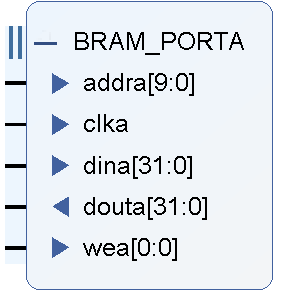
\includegraphics[width=0.2\textwidth]{ip.png}
    \caption{BMG ip核}
    % \label{fig:my_label}
\end{figure}

\begin{enumerate}
    \item addra : 10位指令存储器地址
    \item clka  : 时钟信号
    \item dina  : 32位写输入
    \item douta : 32位读输出
    \item wea   : 0位写使能信号
\end{enumerate}


\newpage
\section{实验过程记录}
\subsection{ALU}
\begin{enumerate}
    \item 使用组合逻辑实现ALU,其中包括加、减、与、或、非、SLT六种运算。在仿真和上板过程中均验证ALU设计功能正常。
\end{enumerate}

\subsection{阻塞流水线加法器}
\begin{enumerate}
    \item 实现了4级流水线32bit全加器,每一级进行8bit加法运算且带有流水线暂停和刷新。
    \item 使用四个always语句块形成四级流水线
    \item 第一级:做[7:0]位与进位位的加法操作,并将运算结果和操作数AB传给下一级。
    \item 第二级:做[15:8]位与进位位的加法操作,并将本级运算结果和操作数AB传给下一级。
    \item 第三级:做[23:16]位与进位位的加法操作,并将运算结果和操作数AB传给下一级。
    \item 第四级:做[31:24]位与进位位的加法操作,并将结果组合输出。
    \item 经仿真验证,如后图,所设计流水线全加器功能正常。
\end{enumerate}

\subsection{问题1:Verilog语法问题和vivado操作问题}
\textbf{问题描述:}由于较长时间未使用Verilog语言和vivado,导致语法和软件操作生疏,具体有无符号拓展时语法报错,仿真时出错。

\textbf{解决方案:}自行复习拼接操作符的使用规范,发现是忘了在最后加上大括号而报错;仿真时未将文件设为顶层而无法完成仿真操作。

\subsection{问题2:流水线加法器仿真图不正确}
\textbf{问题描述:}具体有两种情况,一是运算结果并不是在第四个周期后得出,而是该周期立即得出;二是各级流水线并未存储上一级流水线未参与计算的数据,导致每一级流水线操作数混乱,运算结果出错。

\textbf{解决方案:}第一种情况应该是没有流水线的效果,重新编写为带流水线的加法器;第二种情况因为没有存储各级流水线未参与计算的数据,导致每一级流水线都是加上最新的操作数的各数位,重现添加寄存器存储上一级流水线参与运算的操作数即可。

\newpage
\section{实验结果及分析}
\subsection{ALU验证实验结果}
8位num1输入后无符号拓展为32位
\begin{table}[htbp]
    \centering
    \caption{ALU结果表}
    \begin{tabular}{c|c|c}
        \hline
        操作            &	Num1        &	Result\\
        \hline
        A + B(Unsigned) &	8’b00000010 & 	32'h00000003\\
        A - B           &	8’b11111111 &	32'h000000FE\\
        A AND B         &	8’b11111110 &	32'h00000000\\
        A OR B          &	8’b10101010 &	32'h000000AB\\
        $\overline{A}$  &	8’b11110000 &	32'hFFFFFF0F\\
        SLT             &	8’b10000001 &	32'h00000000\\
        \hline
    \end{tabular}
    \label{tab:my1}
\end{table}

\subsection{流水线阻塞(暂停)仿真图}
\begin{figure}[htbp]
    \centering
    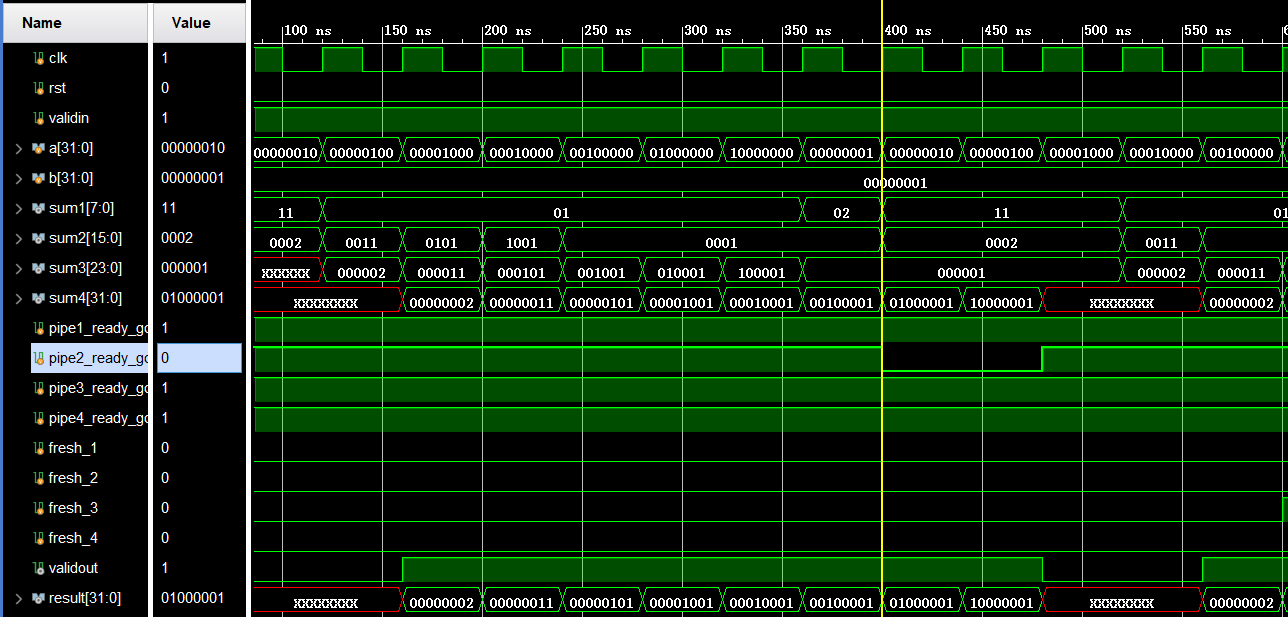
\includegraphics[width=0.9\textwidth]{stop.png}
    \caption{暂停}
    \label{fig:2}
\end{figure}

\subsection{结果分析}
通过该仿真图,我们发现每一个周期,流水线将计算各部分的值,在第四个周期得到最终的运算结果。而第二级暂停时,我们发现第一级流水线也将暂停,保留在一级流水线中的数据不变。第三级,第四级流水线继续运转直到无数据推进,此时,validout信号变为低电平。

\subsection{流水线刷新(清空)仿真图}
\begin{figure}[htbp]
    \centering
    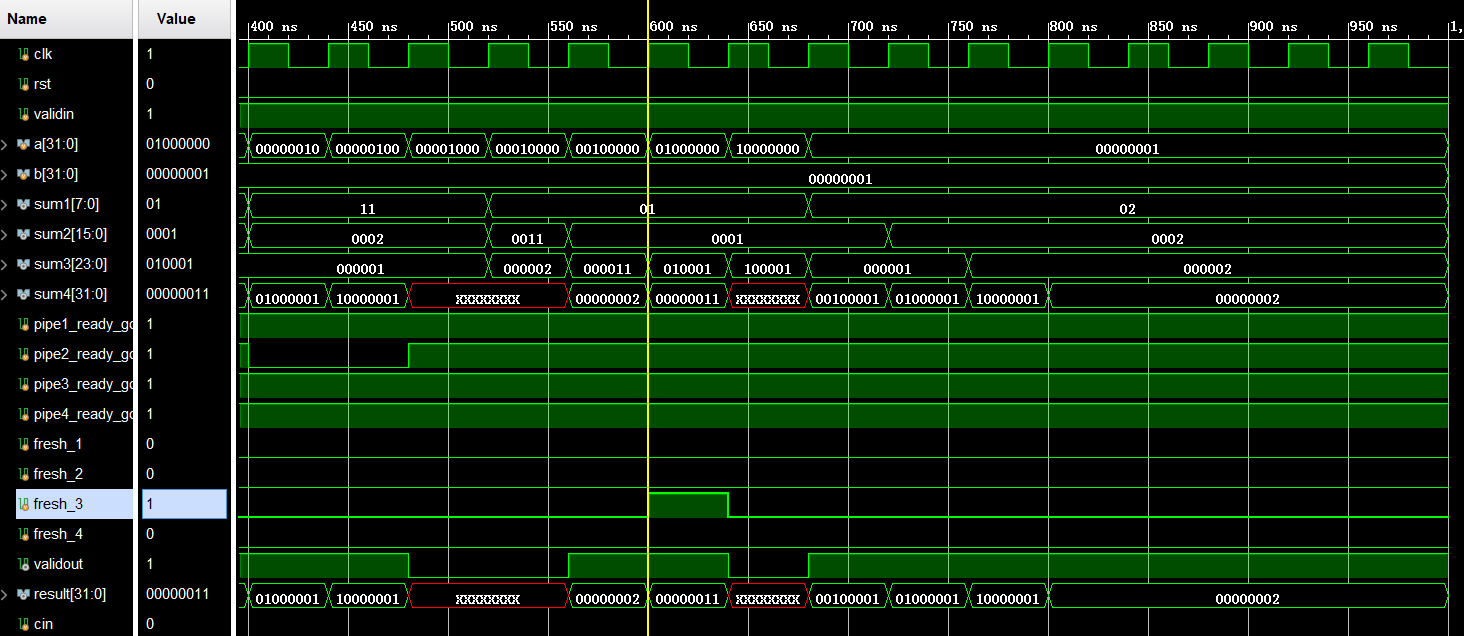
\includegraphics[width=0.9\textwidth]{fresh.png}
    \caption{刷新}
    \label{fig:3}
\end{figure}

\subsection{结果分析}
第三级刷新时,我们发现第一、二级流水线不受影响,但由于第三级流水线的刷新,导致下一周期第四级流水线无法得到数据,此时,validout信号为低电平。

\appendix
\section{Datapath代码}
\begin{lstlisting}[language=Verilog]
    module datapath(
        input clk,
        input reset,
        input memtoreg,
        input pcsrc,
        input branch,
        input alusrc,
        input regdst,
        input regwrite,
        input jump,
        input [2:0]alucontrol,
        output overflow,
        output zero,
        output [31:0] pc, //output pc to inst_ram
        input  [31:0] inst,
        output [31:0] aluout,
        output [31:0] writedata,//write for data_mem
        input  [31:0] readdata //read from data_mem
        );
        
        wire [31:0] pc4;  //pc + 4
        wire [31:0] pc_branch; //branch pc
        wire [31:0] pc_next; // real next pc
        wire [31:0] real_pc; //branch and jump
        
        wire [31:0] ext_imm; //after extension
        wire [31:0] imm_sl2; //after left 2
        
        wire [31:0] result; //real writedata
        wire [31:0] srcB;  //alu operand B
        wire [31:0] srcA;  //alu operand A === RD1
        wire [4:0]  writereg;    //write address
        
        assign pcsrc = branch & zero;
    
        //////////////////////mux//////////////////////////
        mux2 a3_mux(inst[20:16], inst[15:11], regdst, writereg);
        mux2 wd_mux(aluout, readdata, memtoreg, result);
        mux2 srcB_mux(writedata, ext_imm, alusrc, srcB);
        mux2 pc1_mux(pc4, pc_branch, pcsrc, pc_next);
        mux2 pc2_mux(pc_next, {pc4[31:28] , inst[25:0] , 2'b00}, jump, real_pc);
        //////////////////////pc///////////////////////////
        pc counter(clk, reset, real_pc, pc);
        adder pcadder(pc, 32'b100, pc4);   //default add 4
        adder branchadder(imm_sl2, pc4, pc_branch);
        ///////////////////register file///////////////////
        regfile regs(clk, regwrite, inst[25:21], inst[20:16], writereg, result, srcA, writedata);
        ///////////////////signext_imm/////////////////////
        signext sign(inst[15:0], ext_imm);
        /////////////////////sl2///////////////////////////
        sl2 s1(ext_imm, imm_sl2);
        //////////////////////alu//////////////////////////
        alu al(srcA, srcB, alucontrol, zero, overflow, aluout);  //input aluout to data_ram to get readdata
    endmodule
\end{lstlisting}


\end{document}
